% status: 100
% chapter: Swagger REST API

\title{Openstack deployment using Swagger and Libcloud}

\author{Shagufta Pathan}
\affiliation{%
  \institution{Indiana University}
  \city{Bloomington} 
  \state{IN} 
  \postcode{47408}
}
\email{spathan@iu.edu}

% The default list of authors is too long for headers}
\renewcommand{\shortauthors}{Shagufta}

\begin{abstract}
This work focuses on leveraging the capability of Swagger Codegen and Apache 
libcloud for allowing users to easily deploy instances on OpenStack without 
worrying about the underlying architecture. The users can create an instance, 
list instances, add floating ip to the instance, add ssh keypair and more, 
provided the user has permission to perform these activities. Using the REST 
API endpoints, a fully-fledged instance can be created instead of clicking on 
the UI form and filling in the details to get the instance created. We also 
demonstrate the use of cloud-init to send userdata on instance creation by 
executing some basic shell commands. To achieve this, we choose OpenStack as 
the cloud infrastructure since it is ever-growing and one of the most popular 
cloud platform.
\end{abstract}

\keywords{hid-sp18-516, Swagger, REST, Apache libcloud, Python}

\maketitle
\section{Introduction}
OpenStack is an open-source cloud-computing service and is available for free
that provides virtual servers and resources to customers. It is mostly 
deployed as infrastructure-as-a-service~\cite{hid-sp18-516-www-openstack}. 
Whereas Apache Libcloud is a Python library that allows to interact with 
several popular cloud service providers with the help of a unified API to 
interact with different cloud services. The compute component of libcloud 
allows to manage cloud and virtual servers offered by different 
providers~\cite{hid-sp18-516-www-libcloud}. Libcloud helps users to deploy one 
or more virtual machines on OpenStack and allows to run commands on the 
virtual machines. The motivation behind using Libcloud is to ensure that the 
application is portable in terms of the cloud service provider without having 
to rewrite the Swagger specification file.

Figure~\ref{fig:project-architecture} shows the high level architecture. The 
application consists of a REST server implemented using Swagger. The server
provides several APIs which allow provisioning and manipulation of different
resources on the OpenStack cloud. This implementation of the REST server uses 
libcloud to abstract the communication with the cloud. 

\begin{figure}[!ht]
        \centering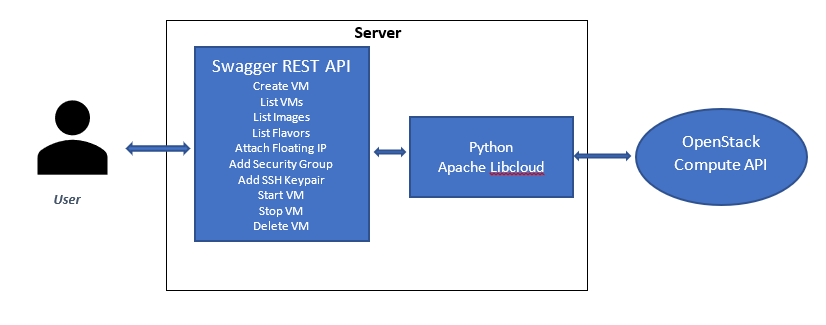
\includegraphics[width=\columnwidth]
        {images/proj-architecture.PNG}
        \caption{Project Architecture}\label{fig:project-architecture}
\end{figure}

\section{Technologies Used}
This section lists the technologies that were used:
\begin{itemize}
\item Python 2.7
\item OpenStack 
\item Swagger Codegen 2.0
\item Apache Libcloud 2.3.0
\item Chameleon Cloud/Horizon
\end{itemize}

\section{Background on Technologies Used}

\subsection{OpenStack}
OpenStack is a set of software tools to build and manage public and private
clouds using pooled virtual resources. OpenStack, managed by OpenStack
Foundation, controls large pools of compute, storage and networking resources
throughout a datacenter. OpenStack is available to users via OpenStack API,
web-based dashboard or through RESTful web
services~\cite{hid-sp18-516-www-wiki-openstack}. It allows users to easily 
deploy virtual machines that can handle a variety of tasks to manage a cloud
environment on the fly. OpenStack is made up of a number of components. But
there are mainly 9 key components~\cite{hid-sp18-516-www-opensource}:

\begin{description}
   \item[Nova:] This is the cloud computing fabric controller, which is the
   main part of an IaaS system. It is used for managing and deploying large
   number of instances to handle computing tasks. 
   \item[Swift:] This is the object Storage system which is scalable
   horizontally by simply adding new servers. It stores files and objects on
   multiple disk drives and OpenStack is responsible for ensuring data
   replication and integrity. 
   \item[Cinder:] This provides block-level storage with OpenStack Compute
   Instances and is important in scenarios where data access speed is the most
   important consideration. 
   \item[Neutron:] This provides networking capability for all the
   OpenStack components and ensures that each component is able to communicate
   effectively and efficiently. 
   \item[Horizon:] This is the dashboard and the only GUI to OpenStack. It
   allows system administrators to easily see what is going on in the cloud and
   manage it as needed.  
   \item[Keystone:] This maintains authentication service across the cloud
   operating system and manages a central directory of users mapping to the
   OpenStack services that they can access. It supports different types of
   authentications including username and password credentials, token-based and
   AWS style logins.
   \item[Glance:] This provides image services to OpenStack and allows
   these images to be used as templates when deploying new virtual machine
   instances. 
   \item[Ceilometer:] This provides telemetry services/billing services to
   individual users of the cloud. It provides all the information on the usage
   reporting which keeps track of user's system of usage of the cloud.
   \item[Heat:] This provides orchestration service that orchestrates
   multiple composite cloud applications using templates. 
\end{description}
	
We focus on using the Compute, Keystone, Horizon and Glance components which 
is made available through the libcloud APIs. 

\subsection{Apache libcloud}
Apache libcloud is a Python library that hides the differences between 
different cloud provider APIs and gives users the ability to manage different 
cloud resources using a unified API. The users do not have to worry about the
underlying architecture of the cloud provider. Libcloud supports more than 50
cloud providers and allows users to manage resources such as the following
categories~\cite{hid-sp18-516-www-libcloud}:

\begin{itemize}
\item Cloud Servers and Block Storage
\item Cloud Object Storage and CDN
\item Load Balancers as a Service
\item DNS as a Service
\item Container Services
\item Backup as a Service
\end{itemize}

For the purposes of this work, we are only going to focus on Cloud Servers
and Block Storage category. Libcloud's compute component that falls under the
Cloud Servers and Block Storage category, can manage cloud and virtual servers
of different cloud providers. Libcloud provides support for Python 2.7, PyPy,
and Python 3~\cite{hid-sp18-516-www-libcloud-compute}. 

Libcloud for OpenStack driver constructor takes different arguments with which
the OpenStack installation can be done. Arguments describing things such as
authentication service API URL, authentication service API version and so on 
can be specified. Note that majority of the arguments to the driver 
constructor are optional~\cite{hid-sp18-516-www-libcloud-openstack}. 

To install the latest stable version of apache-libcloud, open a terminal and
simply run~\cite{hid-sp18-516-www-libcloud}:
\textbf{pip install apache-libcloud}

\subsection{Swagger Codegen}
We use Swagger Codegen 2.0 to design the specifications of the
services developed and to generate the code based on the specifications
developed. Swagger is a tool for developing API specifications based on the
OpenAPI Specification (OAS). It allows not only the specification, but the
generation of code based on the specification in a variety of languages. 
``OpenAPI Specification is an API description format for REST APIs. An OpenAPI 
file can be used to describe the entire API such as available endpoints 
(/users) and operations on each endpoint (GET /users, POST /users), operation 
parameters Input and Output for each operation, Authentication methods and 
contact information, license, terms of use and other
information''~\cite{hid-sp18-516-www-swagger}. 

Swagger Codegen is one of the major swagger tools that is used to generate
server stubs and client libraries from the OpenAPI
specification~\cite{hid-sp18-516-www-swagger}. We are going to use Python
(flask) as the preferred language. The specification is written for OpenStack 
VM deployment and the code has been generated using Swagger Codegen version 
2.0. The same specification can be used for any other provider instead of 
OpenStack as we are using libcloud. The generated code was used to implement 
useful REST APIs using python scripts. Make sure to have Java 7 or 8 installed 
on your system for Swagger Codegen to work. 

\subsection{Chameleon Cloud}
Chameleon is an experimental testbed funded by the NSF FutureCloud program. It
is built over two sites, University of Chicago (UC) and Texas Advanced
Computing Center (TACC). It offers a total of over 550 nodes and 5 PB of space
in twelve Standard Cloud Unit (SCU) racks and about a quarter of the testbed 
is configured with OpenStack KVM. Chameleon provides an installation of 
OpenStack version 2015.1 (Kilo) using the KVM virtualization
technology~\cite{hid-sp18-516-las-handbook}. For the purposes of this work, 
we are going to interact with Chameleon for TACC for monitoring the creation 
of virtual machines and other tasks performed on the VM. The easiest way to 
interact with Chameleon is via the GUI Horizon dashboard as described earlier. 
To log in to the dashboard, we need to have Chameleon username and password 
which can be created on the Chameleon portal. 

\section{Methodology}
We are going to focus on identifying resources related to OpenStack for
deploying an instance of a virtual machine using the REST APIs instead of
using the GUI dashboard by selecting multiple options. The resources 
identified can be considered as part of NIST Big Data Reference 
Architecture (NBDRA). The methodology can be divided into documenting various
resources, using these resources to provide interfaces to access or create
individual resources using the OpenStack libcloud API.

\subsection{NIST Big Data Reference Architecture (NBDRA)}
The NBDRA defines interfaces related to Infrastructure as a Service frameworks.
This includes specific objects useful for OpenStack, Azure, and AWS, as well as
others. It defines different objects that supports functions such as starting,
stopping, suspending, resuming, migration, network configuration, assigning of
resources for the virtual machines~\cite{hid-sp18-516-nist-vol8}. The 
following resources have been identified for interacting with the OpenStack 
framework:

\begin{description}
   \item[List Images:] This service lists all the public and private
   images hosted on Chameleon Cloud. Images contain a virtual disk that has a
   bootable operating system installed on it which are useful for creating
   instances within the cloud. The GET method is used to retrieve all the 
   images of the cloud. 

   \item[List Flavor:] This service lists all flavors/sizes that are
   used to create an instance. Flavors are useful for creating instances within
   the cloud as they define a number of parameters like sizes of RAM, disk,
   number of cores etc\. to specify what type of virtual machine to run. The 
   GET method is used to retrieve all the flavors of the cloud. 

   \item[Create an instance:] This service creates an instance on the
   TACC datacenter of Chameleon cloud. The POST method is used to create an
   instance. The attributes such as instance name, ssh keypair name, security
   group name, flavor id and image id are sent as payload in the POST request.
   Only the instance name is a required parameter, all other parameters are
   picked up from the config file if they are not specified. 

   \item[Import SSH Keypair:] This service allows to import the SSH
   Keypair with the contents of the public key onto OpenStack. Keypairs are SSH
   credentials that are injected into an instance when it is launched. The POST
   method is used to import the SSH Keypair name and Public key file location.
   All the parameters are sent as payload in the JSON format. 

   \item[Attach Floating IP:] This service is used to associate the
   floating IP to the instance from an existing pool of addresses. Once the
   instance is created, in order to access the instance, a floating IP is
   required. An instance has a private, fixed IP address and can also have a
   public or floating IP address. Private IPs are automatically assigned on
   instance creation but need to assign public IPs manually in order to
   communicate with networks outside the cloud, including
   internet~\cite{hid-sp18-516-www-manageips}. POST method is used for this 
   and instance name is sent as payload. 

   \item[Security Group:] This method creates a security group on the
   cloud, if it is not present already. Security group rules are sets of IP
   filter rules that are required as they enable users to ping and use SSH to
   connect to the instance. Security groups define networking access and are
   applied to all instances within a project~\cite{hid-sp18-516-www-secgroup}.
   The security group name is sent as payload in the POST request. 

   \item[Start an instance:] This method starts a stopped instance.
   POST method is used, and instance name is sent as payload. 

   \item[Stop an instance:] This method stops a running instance. POST
   method is used, and instance name is sent as payload. 

   \item[Delete an instance:] This method destroys the specified
   instance. DELETE method is used and instance name is sent as the path
   parameter. 

\end{description}    

\subsection{Swagger RESTful APIs}
The objects described in the above section can be accessed by the REST service
using its own base path. Base paths for the objects of OpenStack will be
\textit{cloudmesh/openstack} followed by the object name. Following shows the
list of APIs developed and implemented inside the Swagger service:

\begin{description}
\item[/images:] lists images available on the cloud
\item[/flavor:] lists the flavors available on the cloud
\item[/listInstances:] lists all the instances available on the cloud
\item[/createInstance:] creates an instance on the cloud
\item[/deleteInstance:] deletes a specified instance
\item[/stopInstance:] stops a specified instance
\item[/startInstance:] starts a specified instance
\item[/addkeypair:] imports the keypair name and content on the cloud
\item[/floatingIP:] associates a floating IP with the specified 
instance
\item[/securitygroup:] creates a security group name with the security
rules 
\end{description}

\subsection{Custom Configuration File}
In order to access OpenStack from libcloud, authentication service API url is
required. This is specified in a configuration file defined as
\textit{class.yaml}. The authentication credentials including username,
password, auth\_url, region\_name, project\_name, version\_number and so on 
can be specified in this yaml file. In order to make the code portable with 
other clouds, different cloud provider details can also be added to this yaml 
file. By default, we only support \textit{TACC} as the cloud provider. 

Reading the configuration parameters from this file and using the REST APIs,
users can easily create instances on the specified cloud without having to
either use the command-line tools or the GUI form to enter the details one by
one. The configuration details entered in the yaml file are obtained by
downloading the environment file called \textit{openrc.sh} file. This file 
provides project-specific details and credentials that the OpenStack services 
can use. It can be downloaded from the web interface via the 
\textit{Access \& Security} link, then clicking on the 
\textit{API Access} tab and clicking on \textit{Download OpenStack RC File} 
on the top of the page~\cite{hid-sp18-516-www-openrc}. 

The class.yaml file used for this work was provided in the class handbook
~\cite{hid-sp18-516-las-handbook}. It has been updated with the latest 
details that are needed for this work. 

\subsection{Using Cloud-Init with OpenStack}
Cloud-init is the Ubuntu package that can handle early initialization of the
cloud instance. It is a set of python scripts and utilities that is installed 
in the Ubuntu Cloud Images. To use cloud-init, we need to use a cloud-init 
enabled image and most Openstack based public cloud providers support it. 
Some of the things it can configure are~\cite{hid-sp18-516-www-cloud-init}:

\begin{itemize}
\item setting up default locale
\item adding ssh keys to user's \textit{.ssh/authorized\_keys} which can 
allow them to log in
\item setting up mount points
\item Configuring network devices
\item setting up a hostname
\item generating ssh private keys
\end{itemize}

Cloud-init can be configured via user-data. User-data can be provided during
instance launch time. User data can be specified in a number of input formats
such as~\cite{hid-sp18-516-www-cloud-init}:

\begin{description}
   \item[Gzip Compressed Content:] Content compressed as gzip data will be
   uncompressed and treated like it were not compressed. Compression of data 
   is useful since there is a limit on the amount of user data that can be 
   sent. It is limited to 16384 bytes. 
   \item[User-Data Script:] This begins with \textit{\#!} or
   \textit{Content-Type: text/x-shellscript}. This script is executed during 
   first boot at \textit{rc.local-like} level, which is very late in the boot 
   sequence. 
   \item[Cloud Config Data:] This content is \textit{cloud-config} data and it
   begins with \textit{\#cloud-config} or 
   \textit{Content-Type: text/cloud-config}. 
   \item[Mime Multi Part archive:] If the user wants to specify more than one
   type of format for example, both user data script and cloud-config, it can 
   be done using this format. 
   \item[Include File:] This file is an \textit{include} file and contains a
   list of urls, one per line. The content read from each of the URLs can be
   gzipped, mime-multi-part or plain-text. It begins with \textit{\#include} or
   \textit{Content-Type: text/x-include-url}. 
   \item[Upstart Job:] Like any other upstart job, the content is placed into a
   file in /etc/init and will be consumed by upstart. This format begins with
   \textit{\#upstart-job} or \textit{Content-Type: text/upstart-job}. 
   \item[Cloud Boothook:] This begins with \textit{\#cloud-boothook} or
   \textit{Content-Type: text/cloud-boothook}. This is the earliest hook 
   available. The content is placed under /var/lib/cloud and then executed 
   immediately. 
   \item[Part Handler:] This is a \textit{part-handler} and begins with
   \textit{\#part-handler} or \textit{Content-Type: text/part-handler}. The 
   content is python code that contains a list\_types method and a 
   handle\_type method and is written to a file in /var/lib/cloud/data 
   based on its filename. 
\end{description}

We are going to demonstrate the use of user data via user-data script. 
Libcloud for OpenStack allows to use cloud-init using the 
\textit{ex\_config\_drive} and \textit{ex\_userdata} arguments to 
create\_node function. The user data we are demonstrating is a list of 
shell commands that will be executed on instance creation and the result 
is saved to an output file called \textit{output.txt} in the user's home 
directory. This userdata is configured in the util.py file.

Following is an example showing how the cloud-init arguments can be provided 
in the libcloud create\_node function:

\begin{figure}[htb]
\begin{verbatim}

userdata = ```#!/bin/bash
echo 'System Information: $(uname -a)' | tee /home/cc/output.txt
echo 'The time is now $(date -R)!' | tee -a /home/cc/output.txt
echo 'The hostname is $(hostname)' | tee -a /home/cc/output.txt
echo 'ifconfig details: $(ifconfig)' | tee -a /home/cc/output.txt
'''
node = driver.create_node(name='vm_name', image=image, size=size,
                          ex_userdata=userdata, ex_config_drive=True)
\end{verbatim}
\caption{User-Data Scripts
~\cite{hid-sp18-516-www-cloud-init}}\label{c:cloud-init-example1}
\end{figure}

Following is another example of user data using cloud-config format. This
example just installs nginx and starts it when the instance is created.

\begin{figure}[htb]
\begin{verbatim}

cloud_init_config = ```
#cloud-config
packages:
 - nginx
runcmd:
 - service nginx start
'''
node = driver.create_node(name='cloud_init', image=image, size=size,
                          ex_userdata=cloud_init_config, ex_config_drive=True)
\end{verbatim}
\caption{Cloud Config Example
~\cite{hid-sp18-516-www-libcloud-functions}}\label{c:cloud-init-example2}
\end{figure}

As explained above, other user data formats can be sent as cloud-init user 
data. Other cloud-config examples include Including users and groups, adding 
a yum repository, Install and run chef recipes, Setup and run puppet, 
Additional apt configuration etc. Cloud-init can prove to be very useful to 
set up the cloud instances on creation depending on the user's
requirement~\cite{hid-sp18-516-www-cloud-init}.

\subsection{Libcloud functions}
The libcloud libraries for compute object were imported using the following
commands~\ref{c:libcloud-libraries}:
\begin{figure}[htb]

\begin{verbatim}

from libcloud.compute.types import Provider

from libcloud.compute.providers import get_driver

\end{verbatim}

\caption{Libcloud libraries
~\cite{hid-sp18-516-www-libcloud-functions}}\label{c:libcloud-libraries}

\end{figure}

The following table~\ref{tab:Description} lists the libcloud functions that 
were leveraged during the development of the REST 
APIs~\cite{hid-sp18-516-www-libcloud-functions}. 

\begin{table}[]
\centering
\caption{Libcloud functions leveraged}\label{tab:Description}
\begin{tabular}{*{2}{c}}
\toprule
Description                      & Function \\
\midrule
To instantiate the driver        & libcloud.get\_driver (Provider.OPENSTACK) \\
To list images                   & list\_images () \\
To list flavor                   & list\_sizes () \\
To list instances                & list\_nodes () \\
To list floating IPs             & ex\_list\_floating\_ips () \\
To list floating IP pools        & ex\_list\_floating\_ip\_pools () \\
Attach floating ip to instance   & ex\_attach\_floating\_ip\_to\_node () \\
To list keypairs                 & list\_key\_pairs () \\
To create security group         & ex\_create\_security\_group () \\
To create security group rules   & ex\_create\_security\_group\_rule () \\
To get image from id 	         & get\_image (img\_id) \\
To get flavor from id            & ex\_get\_size (flvr\_id) \\
To create instance               & create\_node () \\
To delete instance               & destroy\_node () \\
To start instance                & ex\_start\_node () \\
To stop instance                 & ex\_stop\_node () \\
\bottomrule
\end{tabular}
\end{table}

\section{Artifacts}

The Figure~\ref{c:project-artifacts} lists the artifacts provided as part of
this work:
\begin{figure}[htb]
\begin{verbatim}

Makefile
Dockerfile
util.py
default_controller.py
openstack.yaml
class.yaml
requirements.txt
\end{verbatim}
\caption{Project Artifacts}\label{c:project-artifacts}
\end{figure}

Code details
\begin{description}

\item \textit{Makefile}: Makefile contains different targets that perform
different tasks like generate Swagger server-side code, copy files to the
desired location, start and stop the Swagger service, import required packages
for the REST services code, test different Swagger REST APIs, build docker
image, run the docker container, start and stop the docker container.

\item \textit{Dockerfile}: Dockerfile contains all the requirements needed to
build the docker image such as installing Ubuntu, python 2.7, setting up pyenv,
downloading swagger-codegen jar file, setting up the work directory, copying 
all the files to the desired work directory and starting the swagger service. 

\item \textit{openstack.yaml}: This is a yaml document file which contains the
definitions of the REST services for OpenStack deployment conforming to
Swagger/OpenAPI 2.0.

\item \textit{class.yaml}: This file contains the authentication information 
and other configuration details related to OpenStack. As some information like
username, password is sensitive information, it needs to be
configured in this file before execution. Default parameters for image, flavor,
security group, keypair name can also be specified in this file.

\item \textit{util.py}: python script for reading the configurations from
class.yaml and cloud-init configuration for OpenStack.

\item \textit{default\_controller.py}: This is a Swagger controller file with
the actual implementation of the REST services for OpenStack.

\item \textit{requirements.txt}: This file lists all the dependency python
packages that are needed for execution.
\end{description}

\section{Results}
The Swagger REST services can be deployed as a standalone service or as a 
docker container using the commands specified in the Makefile. The service 
can be accessed through browser or CURL utility to verify the execution. After 
running each test target specified in the Makefile (test\_VMs, test\_images,
test\_flavors, test\_createVM etc.), we can log on to Chameleon cloud to 
verify and validate the result. Some screenshots of the test execution have 
been provided. 

Figure~\ref{fig:list-images} shows the execution of the REST API for listing
images of OpenStack available on the Chameleon cloud. As you can see, all the
images, both public and private that are available on the cloud for OpenStack
have been listed.

\begin{figure}[!ht]
        \centering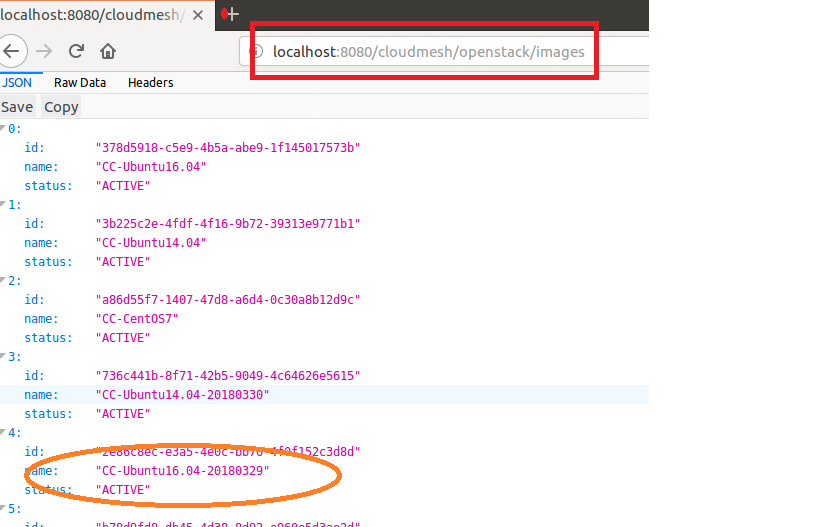
\includegraphics[width=\columnwidth]{images/images.png}
        \caption{List Images}\label{fig:list-images}
\end{figure}

Figure~\ref{fig:list-flavors} shows the execution of the REST API for listing
flavors of OpenStack available on the Chameleon cloud. As you can, all the 
flavors that are needed for instance creation are listed, and the user can 
choose any flavor from this list that is required for creating the instance.  

\begin{figure}[!ht]
        \centering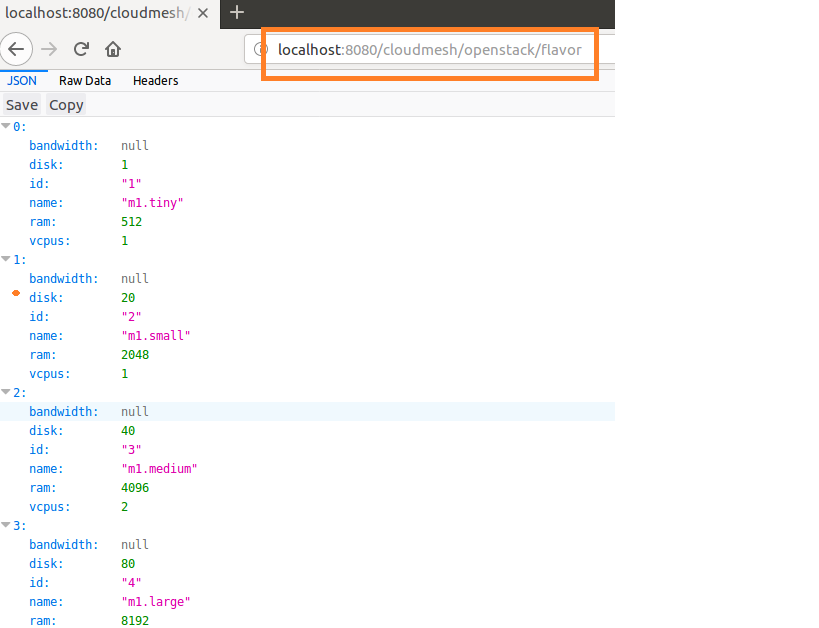
\includegraphics[width=\columnwidth]{images/flavors.png}
        \caption{List Flavors}\label{fig:list-flavors}
\end{figure}

Figure~\ref{fig:createVM} shows the execution of the REST API for creating
instances and its availability on Chameleon cloud. As you can see, we were
able to successfully create two instances \textit{test-VM1-516} and 
\textit{test-VM2-516} and verify that it is listed on the UI.

\begin{figure}[!ht]
        \centering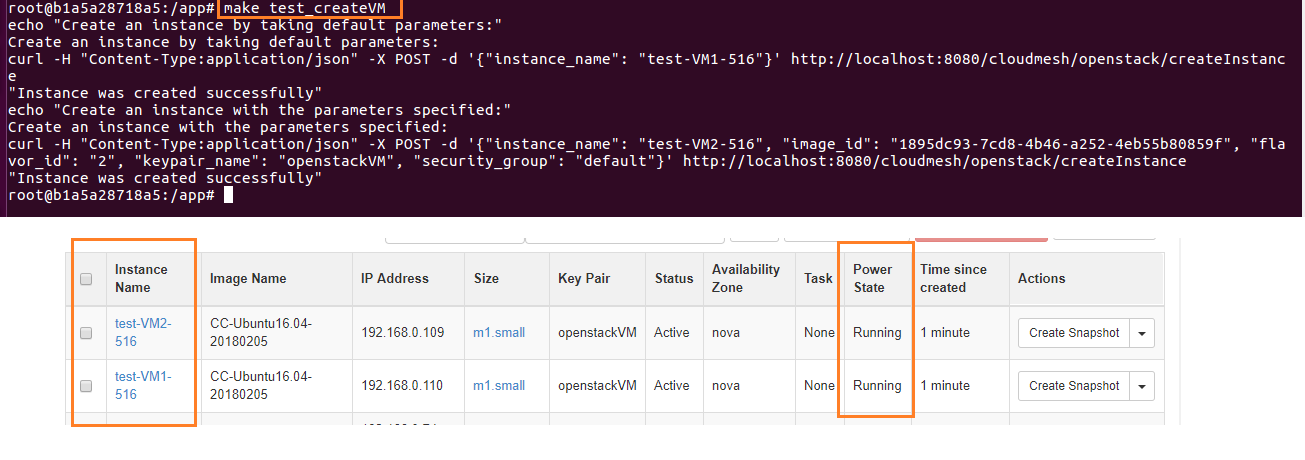
\includegraphics[width=\columnwidth]{images/createVM.png}
        \caption{Create Instance}\label{fig:createVM}
\end{figure}

Figure~\ref{fig:listVM} shows the execution of the REST API for listing all 
the instances of OpenStack available on the Chameleon cloud. As you can see, 
all the instances that have been created by different users are listed, 
including the ones we created previously. 

\begin{figure}[!ht]
        \centering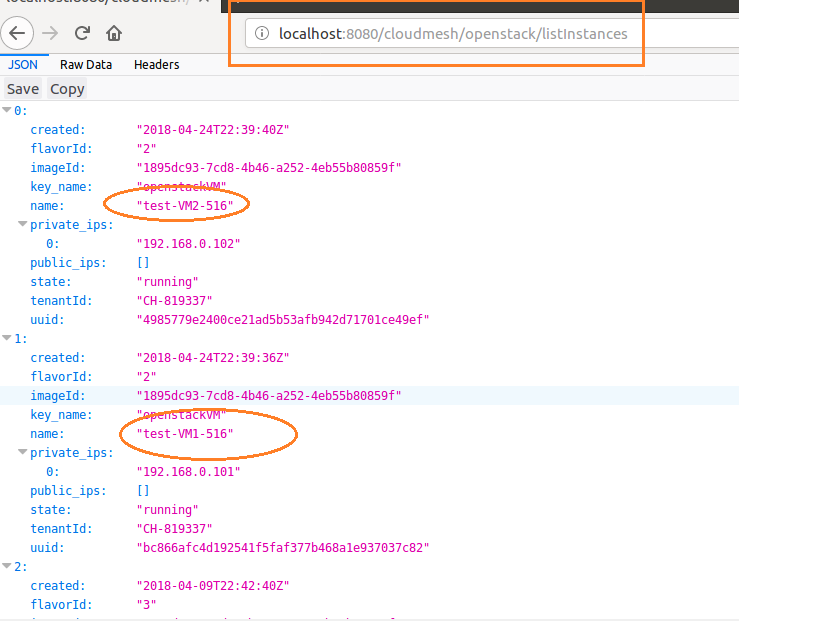
\includegraphics[width=\columnwidth]{images/listVMs.png}
        \caption{List VMs}\label{fig:listVM}
\end{figure}

Figure~\ref{fig:floatingIP} shows the execution of the REST API for associating
floating IP of instance \textit{test-VM2-516} and its result on Chameleon 
cloud. By default, only private IP is assigned on instance creation, assigning
floating IP will allow user to access it outside the cloud. 

\begin{figure}[!ht]
        \centering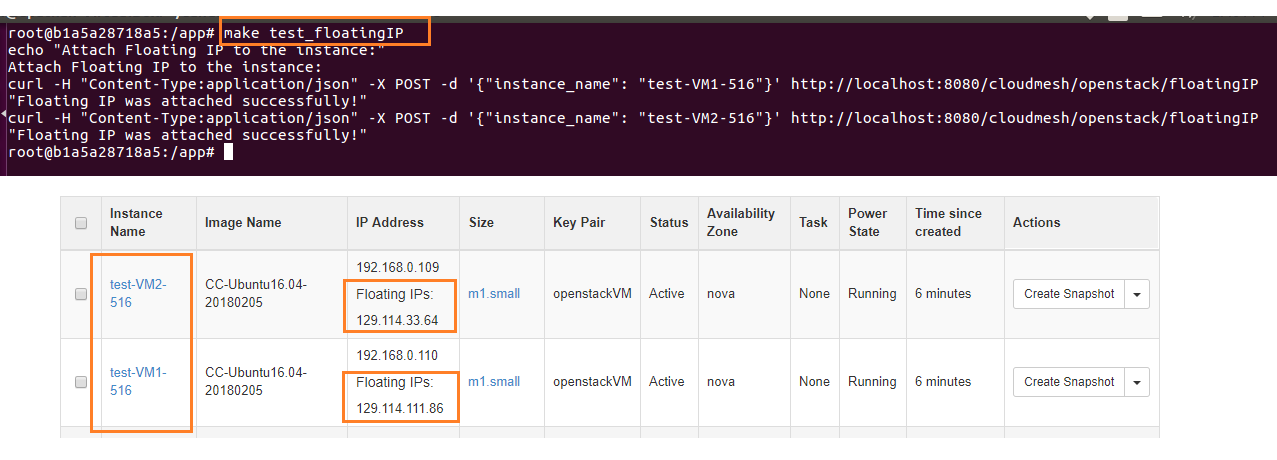
\includegraphics[width=\columnwidth]{images/floatingip.png}
        \caption{Floating IP}\label{fig:floatingIP}
\end{figure}

Figure~\ref{fig:deleteVM} shows the execution of the REST API for deleting
instance of OpenStack. Listing all the instances again should not display the
deleted instance.
\begin{figure}[!ht]
        \centering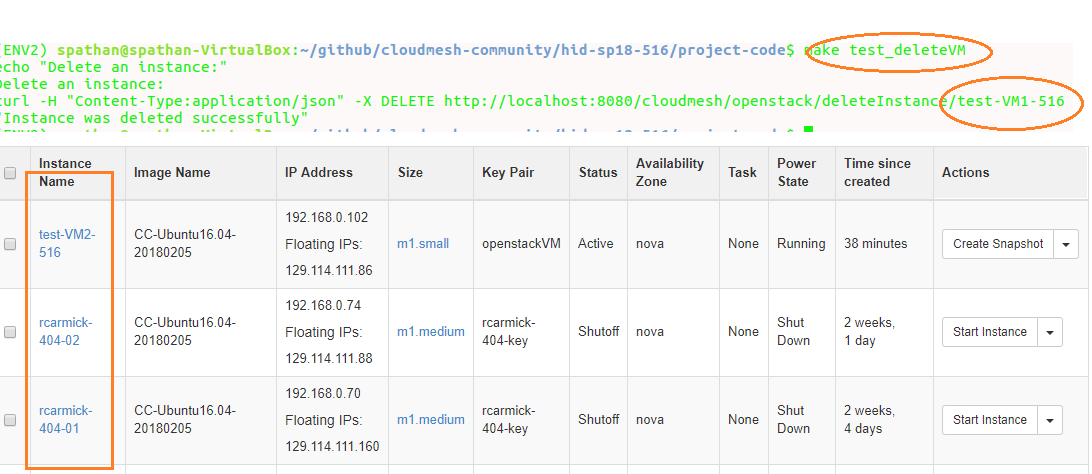
\includegraphics[width=\columnwidth]{images/deleteVM.png}
        \caption{Delete Instance}\label{fig:deleteVM}
\end{figure}

Figure~\ref{fig:stopVM} shows the execution of the REST API for stopping
instance of OpenStack and its result on the Chameleon cloud. Once the instance
is stopped, you can check its status on the UI. It should display 
\textit{Shutoff} against the instance name. Or you can also list the instances
again and check its status.

\begin{figure}[!ht]
        \centering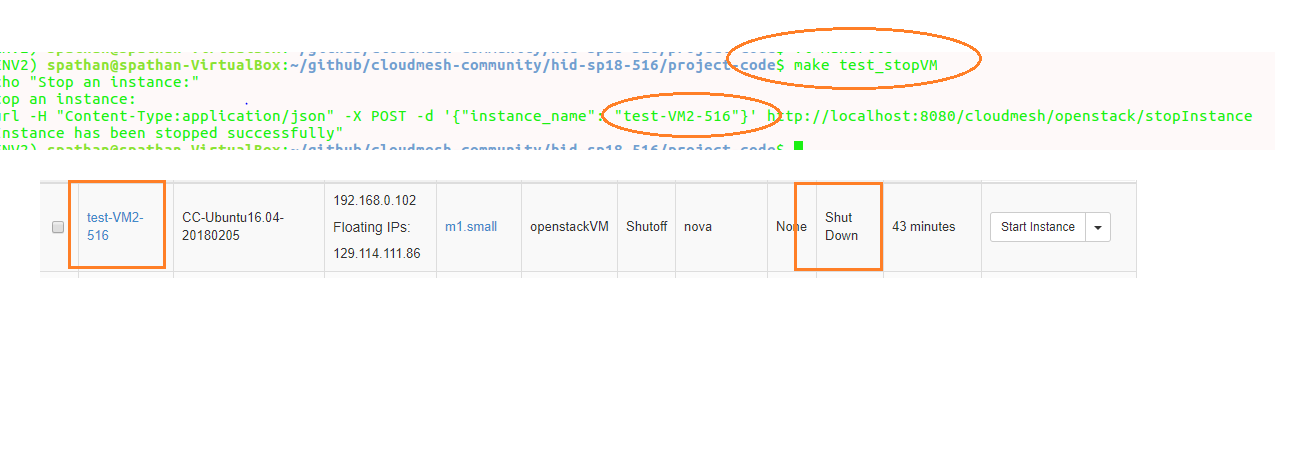
\includegraphics[width=\columnwidth]{images/stopVM.png}
        \caption{Shut Off Instance}\label{fig:stopVM}
\end{figure}

Once the instance is up and running, we can log in to that instance via
\textit{ssh} using the floating IP associated with the instance. The user
\textit{cc} allows automatic login to the instance. We have a REST API that
allows associating floating IP to the instance as seen in the screenshots shown
earlier. Following is the command to login to the instance:
\textit{ssh cc@floatingIPofVM}

Once logged in, we can navigate to /home/cc/ and view the output of the 
commands executed via cloud-init. The result is saved in output.txt.

A short video explaining the execution details of this work has been
created and the link has been added to the README.md file present inside the  
project-code folder.

\section{Conclusion}
We were able to successfully show how the OpenStack instances can be deployed 
using Apache libcloud with the help of Swagger generated code. We showed how 
Apache libcloud can be leveraged to perform different tasks like 
create/delete/start/stop instances or attach floating IP and so on on the 
OpenStack cloud using the unified API abstracting away the underlying details 
of the cloud provider. We also demonstrated how the userdata can be sent on 
the cloud during instance creation using cloud-init configuration and how it 
can be used to perform different user-defined tasks. All this was achieved 
with the help of python scripts that leveraged libcloud into RESTful APIs 
using the Swagger specifications that was created in OpenAPI format. 
Currently, we are using TACC as the default testbed for interacting with 
Chameleon cloud. A substantial future work would be take input from user to 
specify on which testbed/cloud the user would like to deploy their instances. 

\begin{acks}

  The author would like to thank Dr.~Gregor~von~Laszewski for his
  support and suggestions to write this paper.

\end{acks}

\bibliographystyle{ACM-Reference-Format}
\bibliography{report} 

